\documentclass[10pt,a4paper]{article}
\usepackage[margin=1.7cm]{geometry}
\usepackage{amsmath,amssymb}
\usepackage{booktabs}
\usepackage{array}
\usepackage{xcolor}
\usepackage{enumitem}
\usepackage[hidelinks]{hyperref}
\usepackage{caption}
\usepackage{titlesec}
\usepackage{float}
\usepackage{tikz}
\usetikzlibrary{arrows.meta,positioning,fit,backgrounds,calc}
\usepackage{pgfplots}
\pgfplotsset{compat=1.17}
\usepgfplotslibrary{fillbetween,groupplots}

\titlespacing*{\section}{0pt}{7pt}{2pt}
\titleformat{\section}{\normalfont\normalsize\bfseries}{\thesection}{0.5em}{}
\setlist{nosep,leftmargin=1.2em}
\captionsetup{font=footnotesize,skip=3pt}
\pagestyle{plain}
\setlength{\parskip}{3pt}
\setlength{\parindent}{0pt}
\renewcommand{\arraystretch}{1.0}
\newcommand{\F}[1]{\textcolor{blue!55!black}{\footnotesize[#1]}}
\definecolor{ctrl}{HTML}{34A853}
\definecolor{cell}{HTML}{BDC1C6}
\definecolor{offc}{HTML}{E8F0FE}
\definecolor{onc}{HTML}{E6F4EA}
\definecolor{gate}{HTML}{FEF7E0}
\definecolor{todo}{HTML}{F1F3F4}
\definecolor{done}{HTML}{CEEAD6}

\begin{document}

\begin{center}
{\Large\textbf{CS4.406 Term Project --- Mid-Submission Report}}\\[2pt]
{\large\textbf{How fast does a news recommender go stale?}}\\[2pt]
{\normalsize Noel Alex Jacob (2025201085) \quad Emil Joji (2025201040) \quad Kspsvln Siddardha Kumar Kavuri (2025201061)}
\end{center}

\section{What we are studying}
A news recommender learns from past clicks and articles, then stays frozen. But news articles are replaced within hours.
We want to know how fast a frozen recommender gets worse, and which kind of signal gets worse first:
\textbf{word matching} (BM25), \textbf{meaning matching} (a frozen multilingual MiniLM model), or \textbf{click history}
(which articles were read by the same people). Recency and popularity are simple baselines.

\textbf{How we measure it.} Take a real click. List the articles published in the 48 hours before it. Rank the clicked article among them (metrics: MRR, and the \textbf{top-10 hit rate}, which is recall@10: the share of clicks where the clicked article lands in the top 10; both with bootstrap confidence intervals).
Do this for models frozen on different days and compare each one with a model rebuilt the day before. The gap is the \emph{decay}.

\section{Data}
\begin{center}
\small
\setlength{\tabcolsep}{5pt}
\begin{tabular}{@{}lrrr@{}}
\toprule
 & \textbf{EB-NeRD} (main) & \textbf{NPR} (second) & \textbf{Adressa} (optional)\\
\midrule
Publisher, language & Ekstra Bladet, Danish & Globo, Portuguese & Norwegian news site\\
Days of clicks & 22 (May 2023) & 118 (Jan--Apr 2023) & 90 (Jan--Mar 2017)\\
Clicks & 113.4\,M & 17.6\,M & 35.2\,M\\
Users & 791,582 & 1,162,802 & 3,614,911\\
Typical age of a clicked article & 1.4\,h & 13.8\,h & 5.8\,h\\
\bottomrule
\end{tabular}
\end{center}
All three were cleaned into small per-day click files inside the project, and the article text was embedded on the GPU.
For EB-NeRD we use the click history of the validation users, because it is the one part whose volume and type of click stay the same across dates.

\section{Pipeline}
\begin{figure}[H]
\centering
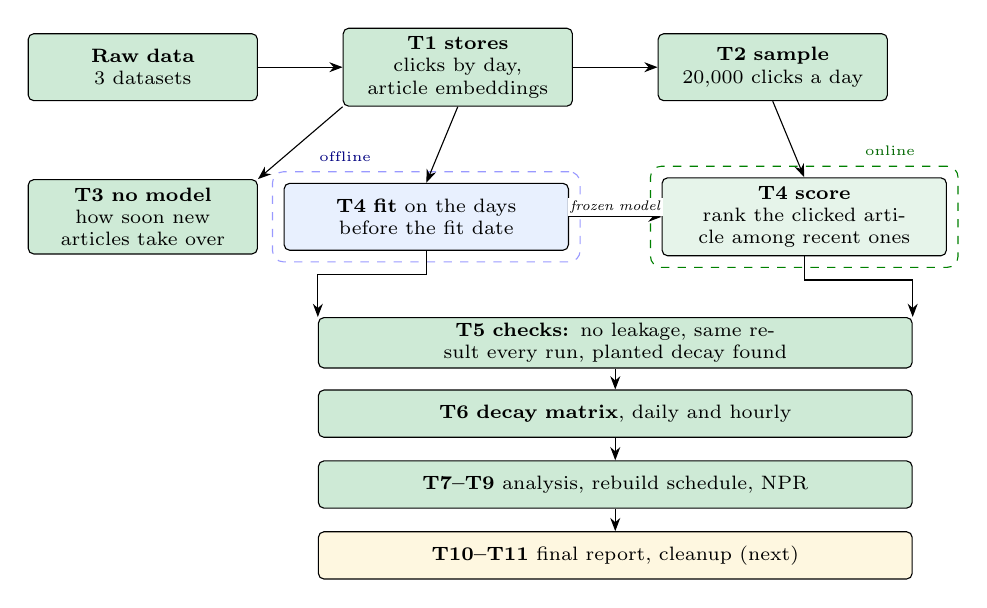
\begin{tikzpicture}[font=\scriptsize, >=Stealth,
  box/.style={draw, rounded corners=2pt, align=center, minimum height=0.85cm, inner sep=3pt, text width=2.7cm},
  wide/.style={draw, rounded corners=2pt, align=center, minimum height=0.6cm, inner sep=2pt, text width=7.4cm},
  lab/.style={font=\tiny\itshape, fill=white, inner sep=1pt}]
\node[box, fill=done] (raw) at (0,0) {\textbf{Raw data}\\3 datasets};
\node[box, fill=done] (store) at (4.0,0) {\textbf{T1 stores}\\clicks by day, article embeddings};
\node[box, fill=done] (samp) at (8.0,0) {\textbf{T2 sample}\\20,000 clicks a day};
\node[box, fill=done] (mf) at (0,-1.9) {\textbf{T3 no model}\\how soon new articles take over};
\node[box, fill=offc, text width=3.4cm] (fit) at (3.6,-1.9) {\textbf{T4 fit} on the days before the fit date};
\node[box, fill=onc, text width=3.4cm] (score) at (8.4,-1.9) {\textbf{T4 score}\\rank the clicked article among recent ones};
\node[wide, fill=done] (t5) at (6.0,-3.5) {\textbf{T5 checks:} no leakage, same result every run, planted decay found};
\node[wide, fill=done] (mat) at (6.0,-4.4) {\textbf{T6 decay matrix}, daily and hourly};
\node[wide, fill=done] (an) at (6.0,-5.3) {\textbf{T7--T9} analysis, rebuild schedule, NPR};
\node[wide, fill=gate] (rep) at (6.0,-6.2) {\textbf{T10--T11} final report, cleanup (next)};
\draw[->] (raw) -- (store);
\draw[->] (store) -- (samp);
\draw[->] (store.south) -- (fit.north);
\draw[->] (samp.south) -- (score.north);
\draw[->] (store.south west) -- (mf.north east);
\draw[->] (fit.east) -- node[lab, above]{frozen model} (score.west);
\draw[->] (fit.south) -- ++(0,-0.3) -| (t5.north west);
\draw[->] (score.south) -- ++(0,-0.3) -| (t5.north east);
\draw[->] (t5) -- (mat);
\draw[->] (mat) -- (an);
\draw[->] (an) -- (rep);
\begin{scope}[on background layer]
 \node[draw=blue!40, dashed, rounded corners, fit=(fit), inner sep=4pt, label={[font=\tiny, text=blue!50!black]above left:offline}] {};
 \node[draw=green!50!black, dashed, rounded corners, fit=(score), inner sep=4pt, label={[font=\tiny, text=green!40!black]above right:online}] {};
\end{scope}
\end{tikzpicture}
\caption{The pipeline. Green is done, yellow is next. A monitor watches time, memory and disk in every step.}
\label{fig:pipeline}
\end{figure}

\section{What we found}
Stages T1 to T9 are built, and all automated tests pass (including a planted decay that the checks recover). Results on EB-NeRD (14 fit days, about 17,000 clicks a day, 95\% paired bootstrap intervals); ``lag'' is the days since the model was frozen. The user's profile is either \emph{live} (last 50 clicks before the click) or \emph{frozen} (clicks up to the fit date). The hit rates use the live profile:
\begin{center}
\small
\setlength{\tabcolsep}{4pt}
\begin{tabular}{@{}lrrr@{}}
\toprule
 & Top-10 hit rate, lag 1 & Top-10 hit rate, lag 7 & MRR lost by lag 7: frozen / live profile\\
\midrule
Recency (newest first) & 0.515 [0.513, 0.517] & 0.528 [0.525, 0.530] & 0 (by construction)\\
Word matching & 0.061 [0.060, 0.062] & 0.064 [0.063, 0.065] & 0.0030 [0.0024, 0.0036] / 0.0001\\
Meaning matching & 0.047 [0.046, 0.048] & 0.047 [0.046, 0.048] & 0.0007 [0.0003, 0.0011] / 0 (exactly)\\
Random shuffle & 0.027 [0.026, 0.027] & 0.027 [0.027, 0.028] & 0\\
Click history, popularity & 0.008 & 0.027 & \emph{coverage, see below}\\
\bottomrule
\end{tabular}
\end{center}
\begin{itemize}
\item \textbf{Word and meaning matching go stale only through the user's profile.} With a live profile the loss is about 0; with a frozen profile word matching loses 0.0030 [0.0024, 0.0036] MRR by lag 7 (about 10\%) and 0.0059 [0.0047, 0.0071] by lag 13 (about 24\%). They are also weak: 2 to 3 times the shuffle. Recency is far ahead on this news site.
\item \textbf{Click history and popularity fail by coverage, not by accuracy.} At lag 1 they can score only 12\% of the clicked articles, and none at lag 7, because new articles have no clicks yet. Their scores fall to the shuffle level for that reason.
\item \textbf{Hourly:} click history can score 79\% of clicks one hour after the fit, 19\% after 6 hours and 0.9\% after 24 hours. Word matching loses 0.0023 [0.0020, 0.0026] MRR at 24 hours (about 7\% of its score).
\item \textbf{Rebuild interval:} with a live profile, rebuilding word matching daily instead of once gives 0.0325 against 0.0324 MRR, so a rebuild buys almost nothing; with a frozen profile, daily gives 0.0310 and once 0.0274; a click-history rebuild costs 22\,s and about 7\,GB.
\item \textbf{No-model check:} at 6 hours, the share of new clicks that go to unseen articles is \textbf{90.8\%} [88.5, 92.5] for EB-NeRD, \textbf{48.5\%} [45.4, 51.5] for Adressa and \textbf{15.5\%} [11.3, 20.1] for NPR.
\item \textbf{NPR (second dataset)} ranks the signals differently: popularity hit rate 0.550 [0.547, 0.553], click history 0.249 [0.246, 0.251], recency 0.005 [0.004, 0.005]. Popularity gets \emph{better} with an older fit, which we have not yet explained.
\item \textbf{Check without never-clicked articles} (27\% of the articles; this uses future clicks, so it is only a ceiling): every score rises (recency hit rate 0.515 to 0.634 [0.632, 0.636]), but the staleness loss does not change (word matching, live profile, 0.00013 to 0.00010 [0.00003, 0.00016] MRR at lag 7).
\end{itemize}

\section{What went wrong, and what we changed}
\begin{itemize}
\item Our first full run counted articles the user had already read. Our own check found that 15\% of clicks were re-reads, which inflated word matching (MRR 0.057 instead of 0.014 without them). We deleted all results, dropped re-reads and the user's read articles from every pool, and reran everything.
\item The click-history model needed 7.1\,GB, not the 1.5\,GB we planned, so only 2 can run at a time.
\item Two hourly units were marked complete but had missing files. We found it when the analysis failed, and recomputed them.
\end{itemize}

\section{Remaining work}
Final report and AI log (T10), cleanup and a frozen copy of the results (T11). Not done: a hybrid model that falls back to recency when the others cannot score, Adressa, and the cause of popularity improving with an older fit on NPR.

\end{document}
